\documentclass[10pt,a4paper]{article}

\usepackage[utf8]{inputenc}
\usepackage[english]{babel}
\usepackage[english]{isodate}
\usepackage[parfill]{parskip}

\usepackage{forest}
\usepackage{listings}
\usepackage{longtable}
\usepackage{url}
\usepackage[numbers]{natbib}
\usepackage{graphicx}

\pagenumbering{arabic}

\begin{document}

\section{Introduction}

This software generates a list of candidate detections for an input
asteroid population and a list of telescope field pointings.

\section{Installation}

The software has been tested with Python 3 on MacOS and Linux.

Requirements:\\
- python 3\\
- spiceypy python library\\
- pyoorb python library\\
- other standard python libraries like numpy, pandas, etc.\\
- NAIF SPICE Utilities\\

Setup:\\
- Make sure you can import spiceypy, pyoorb, and other libraries in python.\\
- Make sure you can run the NAIF SPICE Utility executables from your command line.\\
- Download the package and run the DownloadKernels.sh script in the kernels/ folder.\\
- Copy the binary de430.dat file required by pyoorb into the data/ folder.\\

The directory structure is as follows:\\

\begin{forest}
  for tree={
    font=\ttfamily,
    grow'=0,
    child anchor=west,
    parent anchor=south,
    anchor=west,
    calign=first,
    edge path={
      \noexpand\path [draw, \forestoption{edge}]
      (!u.south west) +(7.5pt,0) |- node[fill,inner sep=1.25pt] {} (.child anchor)\forestoption{edge label};
    },
    before typesetting nodes={
      if n=1
        {insert before={[,phantom]}}
        {}
    },
    fit=band,
    before computing xy={l=15pt},
  }
[objectsInField
  [code
    [\_\_init\_\_.py]
    [shared.py]
    [sso.py]
    [telescope.py]
    [orbits.py]
    [ooephemerides.py]
  ]
  [kernels
    [...]
  ]
  [data
    [data files]
  ]
  [main
    [context.py]
    [main.py]
    [input.config]
  ]
  [docs
    [manual.pdf]
  ]
]
\end{forest}

An additional directory will be created to store trajectories of
asteroids as SPK files~\citep{spice}.


\section{Usage}

The software should be run from the main directory. The general usage
of the software is: \\

\verb+$ python main.py configfile > output+ \\
or \\
\verb+$ python main.py -f configfile > output+ \\

Here \verb+configfile+ is a file containing all the input parameters
for the simulation. The output can be redirected to a file using the
redirection operator, \verb+>+. By default, the software doesn't
overwrite existing asteroid SPK files unless you use the \verb+-f+
flag. A sample configfile named \verb+input.config+ is provided with
the package.

The descriptions of the various files needed by the software are given
in the subsections that follow.

\subsection{Configfile}

The `configfile' follows the structure used by the \emph{configparser}
module of \emph{Python}. A sample configfile named \verb+input.config+
is provided in the \verb+main+ directory. Briefly, the file is divided
into sections that begin with headers of the form \verb+[SECTION]+,
where \verb+SECTION+ is the name of the section. Each section consists
of multiple lines of the form \verb+keyword = value+.  The
\verb+configfile+ for this software consists of four sections. All
sections are mandatory but some keyword/value pairs are optional.
Table \ref{tab:desc} describes each keyword that the software
accepts. Mandatory fields are denoted by an asterisk (*).

\begin{longtable}{l l p{20mm} p{50mm}}
    \hline
    Keyword                   & Section  & Default value & Description\\
    \hline \hline \\
    \verb+Data path+ *        & CONF         & NA             & Path of the directory where the SPICE meta-kernel,
                                                               the JPL planetary ephemeris file, and the \verb+Population model+ file reside. 
                                                               The software also uses this folder to write the temporary files.\\ \\
                                                               
    \verb+SPICE metakernel+ * & CONF         & NA             & Filename of the NAIF SPICE meta-kernel.
                                                               The meta kernel resides in \verb+Data path+
                                                               and contains paths to
                                                               all the common SPICE Kernels
                                                               required by the software that are
                                                               not survey specific. Read about
                                                               how to prepare the meta-kernels at
                                                               \citep{spice}.\\ \\
                                                   
    \verb+Planetary ephem+ *  & CONF          & NA            & Name of the JPL planetary ephemeris file required
                                                               by OpenOrb \citep{openorb}.\\ \\
                                                   
                                                   
    \verb+nProc+              & CONF          & 1             & (Currently not supported) Number of 
                                                               parallel processes to use. \\ \\
  
    \verb+Camera+ *           & CAMERA        & NA            & Name of the file containing the definition of 
                                                               the camera field of view. File description in Section~\ref{sec:fov}. \\ \\
   
    \verb+SPICE IK+           & CAMERA        & camera.ti     & Filename of the SPICE instrument kernel that 
                                                               the software will write in the \verb+Data path+ folder. \\ \\
 
    \verb+Threshold+          & CAMERA        & 5             & Angular separation threshold in degrees for 
                                                               performing an initial rough search for 
                                                               detectable targets. This threshold should be larger
                                                               than the field of view of the camera. \\ \\ 
                                                   
    \verb+Population model+ * & ASTEROID      & NA            & Name of the file containing the asteroid orbits.
                                                               This file should be in the \verb+Data path+ folder. \\ \\

    \verb+Asteroid SPK path+ *& ASTEROID      & NA            & Path of the directory where all the asteroid SPKs are or will be stored. 
                                                               This path is relative to \verb+Data path+.\\ \\

    \verb+Asteroid SPKs+ *    & ASTEROID      & NA            & Asteroid SPK base filename. The trajectory of each
                                                               asteroid will be saved in a separate SPK file having a filename
                                                               that is the base name appended by an integer and the file extension (.bsp).\\ \\
                                                   
    \verb+Object1+            & ASTEROID      & 1             & Line number of the first asteroid orbit to be read from the 
                                                               \verb+Population model+ file. Should be $>$ 1. \\ \\
 
    \verb+nObjects+           & ASTEROID      & 1             & Number of asteroid orbits to read from the \verb+Population model+ file
                                                               starting from \verb+Object1+. \\ \\

    \verb+Make SPKs+          & ASTEROID      & T             & Flag to indicate whether the asteroid orbits should be propagated 
                                                               and the ephemerides should be saved in SPK files.
                                                               If the appropriate SPK files already exists, set the value to F 
                                                               otherwise set it to T. \\ \\

    \verb+SPK T0+ *           & ASTEROID      & NA            & Start time for generating the asteroids and/or the observatory spks. \\ \\

    \verb+nDays+              & ASTEROID      & 4000          & Required length in days of asteroid and/or observatory spks. \\ \\

    \verb+SPK step+           & ASTEROID      & 20            & Step size to use for generating the asteroid ephemerides. \\ \\

    \verb+nbody+              & ASTEROID      & F             & Type of propagation to generate asteroid SPKs (T for N-body and F for 2-body).
                                                               2-body just includes the Sun. N-body includes the 8 planets and the Moon. \\ \\
    
    \verb+Survey database+ *  & SURVEY        & NA            & Name and path of the sqlite database that contains 
                                                               the field pointing information. The path should be given 
                                                               relative to \verb+Data path+. \\ \\

%    \verb+Survey T0+          & SURVEY        & Read from database & Time-shift the entire survey such that the first exposure time is on 
%                                                                    day\verb+Survey T0+. Fractional day from the database will be preserved. 
%                                                                    \verb+Survey T0+ value must be an integer. \\ \\
                                                                      
    \verb+Field1+             & SURVEY        & 1             & First field to read from the database \\ \\

    \verb+nFields+            & SURVEY        & 1000          & Number of fields to read from the database. 
                                                                If \verb+nFields+ is greater than the number of fields in the database,
                                                                then all fields will be read. \\ \\
                                                                
    \verb+Space+              & SURVEY        & F             & Value of T indicates that the user is simulating a space-based survey.
                                                               If \verb+Space+=T, \verb+SCID+ is required and the 
                                                               spacecraft SPK file (named \verb+SCID.bsp+) must be provided. If \verb+Space+=F,
                                                               \verb+MPCobscode file+ and \verb+Telescope+ are required. \\ \\
  
    \verb+SCID+ $^a$          & SURVEY        & NA            & Integer ID of the spacecraft. Required if \verb+Space+ = T. 
                                                               (See rules on SCID in section xx).\\ \\

    \verb+MPCobscode file+$^b$& SURVEY        & NA            & File containing the MPC observatory codes. Required if \verb+Space+=F.
                                                               File should reside in \verb+Data path+ \\ \\ 

    \verb+Telescope+ $^b$     & SURVEY        & NA            & MPC observatory code of the survey telescope. Required if \verb+Space+=F.\\ \\
\hline \\

\caption{Configfile parameters. * indicates that the field is mandatory. $^a$indicates mandatory if Space = T. $^b$ indicates mandatory if Space = F.}
\label{tab:desc}                                                                   
\end{longtable}


\subsection{Survey database}

The survey database is an LSST OpSim SQLite database or a reduced
version of it with only the necessary fields. At a minimum the database
requires the `ObsHistory' table with the fields described in Table
\ref{tab:sumdesc}.

\begin{longtable}{l l p{20mm} p{50mm}}
    \hline
    Column name                   & Type     & Units   & Description\\
    \hline \hline \\
    observationId                 & integer  & -       & Unique visit identifier. \\ \\
    ra                            & real     & radians & Right Ascension (J2000) of the field center for this visit. \\ \\
    dec                           & real     & radians & Declination (J2000) of the field center for this visit (same as Field.fieldDec).\\ \\
    observationstartMJD           & real     & days    & Modified Julian Date at the start of a visit. \\ \\
    angle                         & real     & radians & The orientation of the sky in the focal plane measured 
                                                         as the angle between North on the sky and the "up" direction 
                                                         in the focal plane. \\ \\
\hline \\


\caption{Survey database `Summary' table.}
\label{tab:sumdesc}                                                                   
\end{longtable}


\subsection{Instrument field of view definition}
\label{sec:fov}
The instrument field of view (FOV) is defined in a plain text file
called the `camera file', which is input via the \verb+Camera+ keyword
in the \verb+configfile+. The first line of the camera file defines
the type of FOV. Currently allowed values are \verb+Circle+ or
\verb+Polygon+.  If the first line is \verb+Circle+, then the
following line is the radius of the circle in degrees. If the first
line is \verb+Polygon+, then the subsequent lines will be the angular
coordinates of the corners of the polygon in degrees.
Figure~\ref{fig:instrument} shows the coordinates for a rectangular
FOV. Each row in the file lists the coordinates of a single
corner. The corners are listed in either clockwise or
counter-clockwise order. For the instrument shown in
Figure~\ref{fig:instrument}, the camera file would be:\\\\

\verb+Polygon+ \\
\verb+x1 y1+ \\
\verb+x2 y2+ \\
\verb+x3 y3+ \\
\verb+x4 y4+ \\\\

The camera file for an instrument with a circular field of view with
half angle of 1.5 degrees would be:\\\\

\verb+Circle+\\
\verb+1.5+\\\\

\begin{figure}
  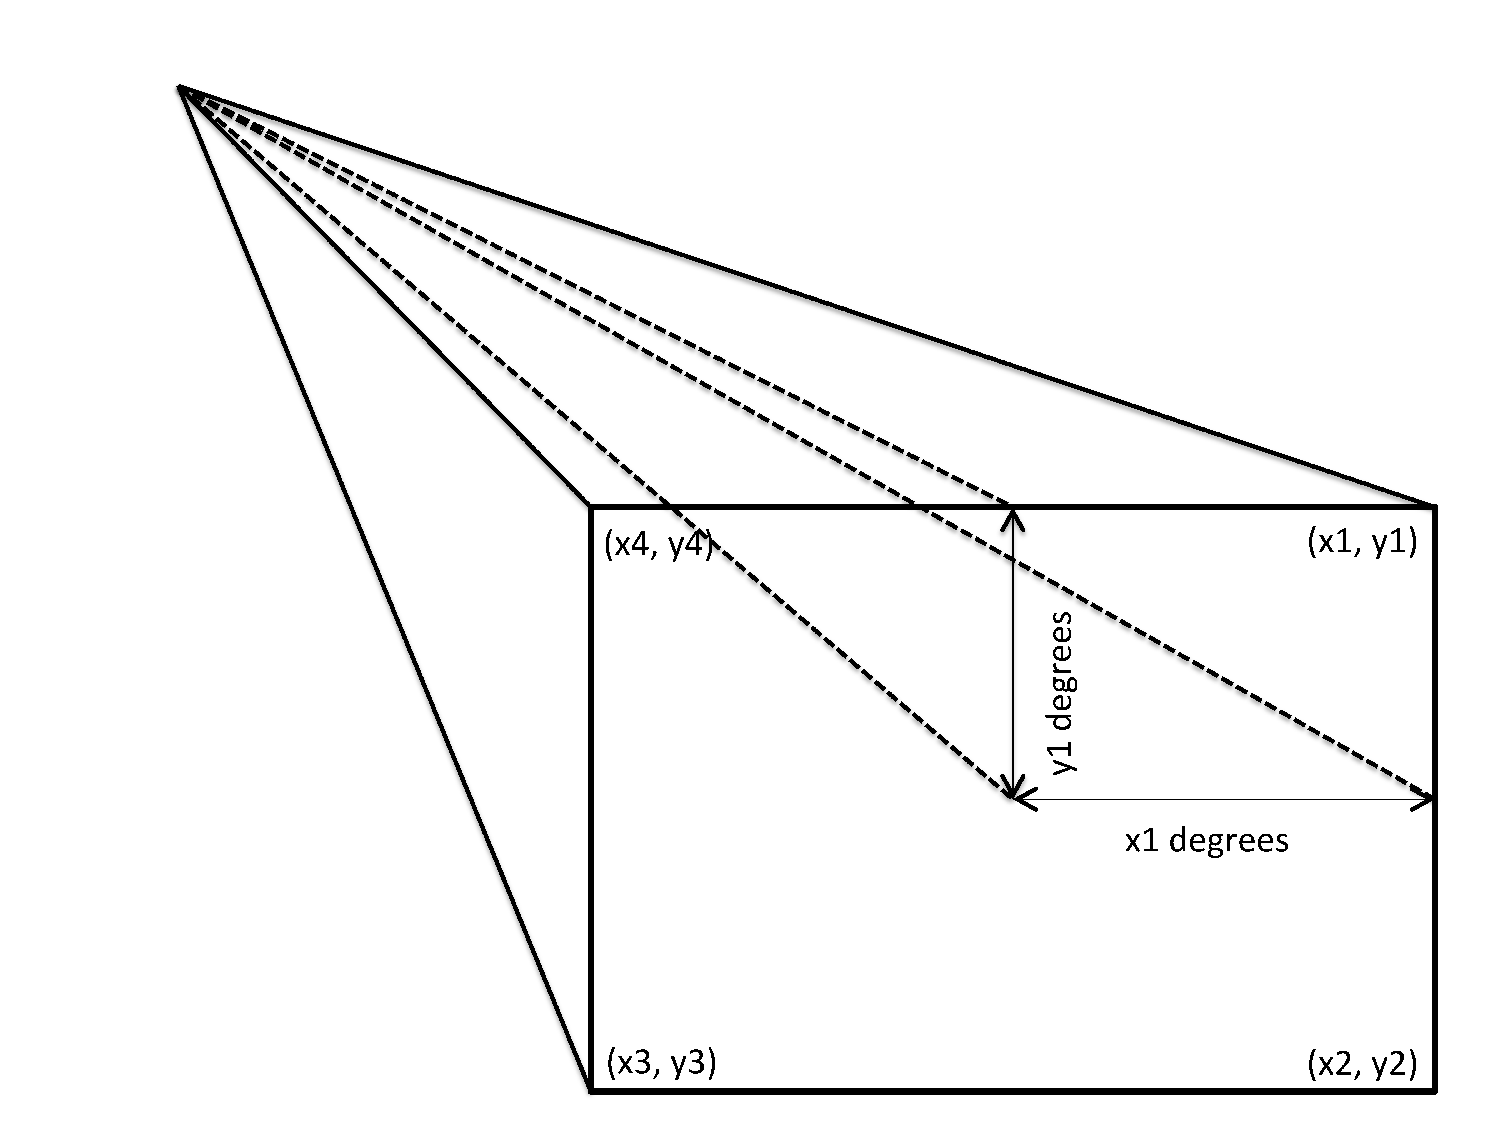
\includegraphics[width=0.8\textwidth]{InstrumentFOV}
  \caption{Coordinates of a rectangular field of view.}
  \label{fig:instrument}
\end{figure}


\subsection{Asteroid population model}
The Asteroid population model file is a plain text file containing a
table of orbital elements in the Ecliptic J2000 frame. The first line
of the file is the header describing the columns,  which can be
in any order. The suggested column names are as follows:

`OID' for Object ID,\\
`FORMAT' for format of elements. Suggested format is `COM' for cometary elements,\\
`q' for perihelion distance in au,\\
`e' for eccentricity,\\
`i' for inclination in degrees,\\
`node' for longitude of ascending node in degrees,\\
`argperi' for argument of pericenter in degrees,\\
`t\_p' for time of pericenter passage in MJD,\\
`t\_0' for epoch of the orbital elements in MJD,\\
`H' for absolute magnitude.\\

Value of OID should be unique for each object.


\newpage
\bibliographystyle{IEEEtran}
\bibliography{manual}
\end{document}


